% !TeX root = ../main.tex

% Homology provides a collection of invariants that represent global properties of a space.
% Under specific assumptions the presence of a property can be assumed when the space itself is largely unknown.
% Then, given a sample of an unknown space satisfying these assumptions, once can use the homology of the sample in order to confirm it is representative of the space with respect to that property.
%
% The Topological Coverage Criterion (TCC) is one example of this technique in which homology can be used in order to verify that a collection of subsets provided by a sample covers the space.
% Specifically, by assuming the top dimensional relative homology is known one can check that of the sample is what we expect in order to certify coverage by relating the top dimensional relative to the boundary of a space to the zero dimensional homology of the complement.

The assumptions made about the boundary are central to the TCC.
While it certainly demonstrates an interesting application of homology to coordinate-free sensor networks these assumptions are unrealistic in practice.
Specifically, it requires that sensors are capable of detecting the physical presence of a boundary.
In a coordinate-free setting, where sensors are unable to measure distance nor communicate their coordinates, this requirement seems unnatural.

Moreover, the efficacy of the condition relies on having enough sensors close enough to approximate the boundary in homology.
As a necessary but not sufficient condition there is room to question what can go wrong in the case of false positives.
We identify this situation in which the ``boundary'' is not sufficiently sampled as one such instance.
This leads us to believe the condition checks for something more specific than coverage alone.

We will re-cast the TCC as a way to verify that a collection of sample points can adequately approximate an unknown function in an unknown space.
Consider the application to sensor networks as an example, where we take our sample points as sensors dropped in an unknown environment.
We now endow our sensors with the ability to measure some unknown quantity that is related to metric of the space in a specific way (Lipschitz).
In this way we can replace the requirement that sensors can detect the presence of the true topological boundary with assumptions about the function itself.
Indeed, these assumptions could relate the behavior of the function to the topological boundary of the space.
However, the condition holds for any subset which ``surrounds'' the space in a specific sense~\cite{cavanna2017when}.

The TCC itself relies heavily on relative homology to use the assumptions made to the homology known.
Specifically, we can confirm coverage of the ``interior'' of the space by effectively quarantining the surrounding space we take homology with respect to.
We take this property of relative homology, which can be understood in terms of excision, to its logical extreme.
We consider the case in which we have incomplete data for a particular sub-levelset of the function.
Returning to our sensor network analogy, suppose our sensors measure heat, or some other volatile quantity, and cannot approach a region without failing.
By properly isolating the region, taken as a sub-levelset of the function, we can confirm that the sample we have is topologically representative of the region near, and above this sub-levelset.
We can then re-use the same machinery that was used to verify coverage to analyze a \emph{part} of the function in a very specific way.

In a superficial sense, the assumptions and machinery required to approximate a function's persistent homology are precisely those confirmed and constructed in the TCC. %\footnote{\textbf{TODON} worst sentence ever, but exactly what I want to say. Also I stole ``superficial'' from your intro because it's perfect. Maybe some of your intro can fill this in.}.
While this approximation is well studied in general~\ref{chazal08towards}, the presence of incomplete data can severely impact the quality of the approximation.
This is primarily due to the nature of homology as a measure of \emph{global} structure.
While the obvious solution is to simply remove the un-verified data, the question of what precisely this would approximate is important to consider.
By simply restricting the function to the verified \emph{super}-levelset we accept that there may be global structure to the function itself that we are missing.
If we are then provided with the missing data it may prove more difficult to reconstruct the full diagram in this case.

% \begin{wrapfigure}{r}{0.5\textwidth}
%   \centering
%   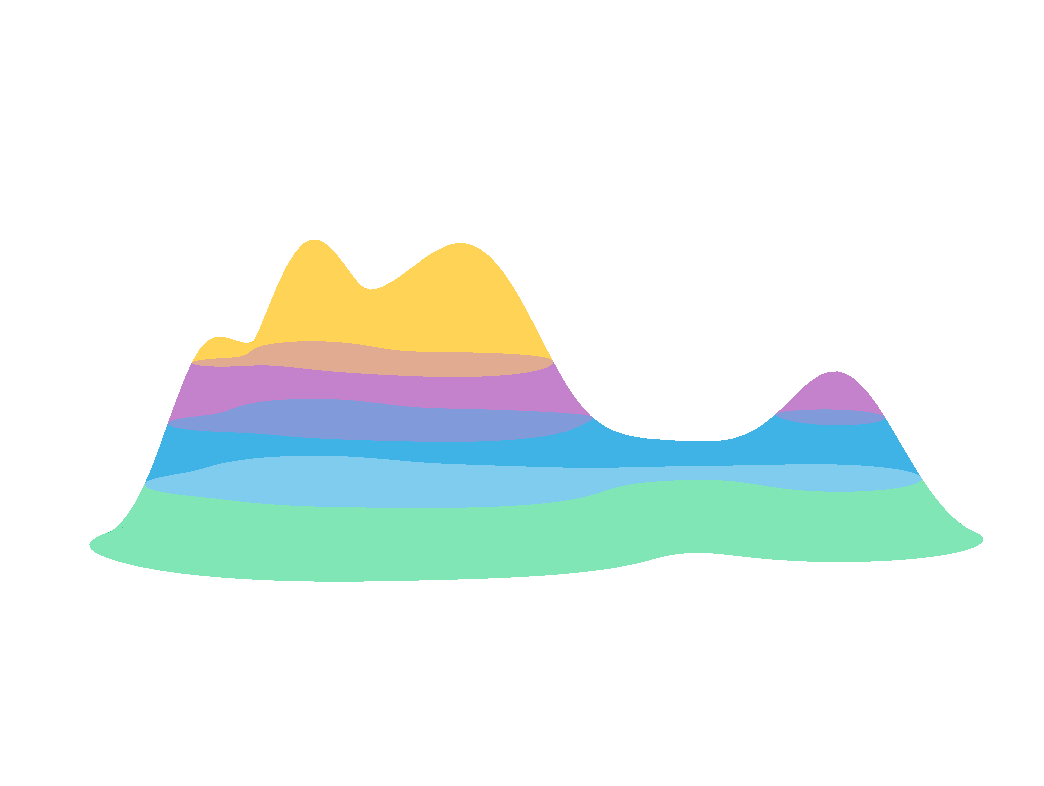
\includegraphics[trim=50 190 0 200, clip, scale=0.2]{scripts/figures/scalar.png}
%   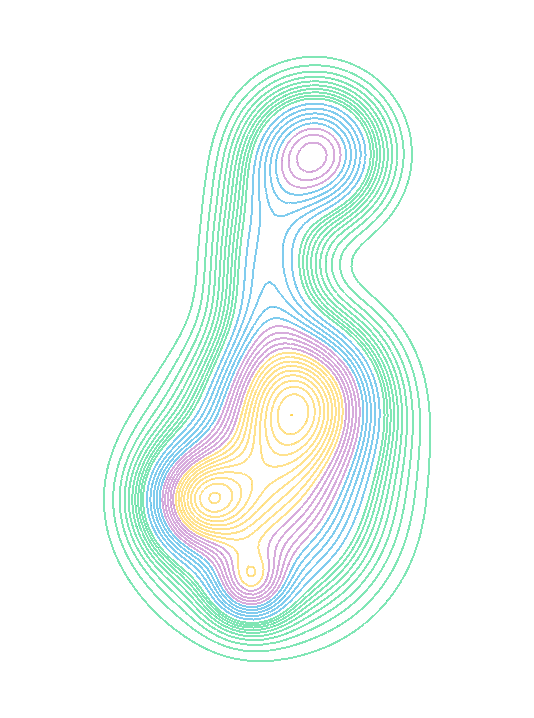
\includegraphics[trim=100 25 75 0, clip, angle=280, scale=0.28]{scripts/figures/scalar_contour.png}
%   % \includegraphics[scale=0.55]{scripts/figures/scalar_barcode_super_0.png}
%   % \includegraphics[scale=0.55]{scripts/figures/scalar_barcode_sub_1.png}
% \end{wrapfigure}

We consider the persistent homology relative to a sub-levelset as a \emph{truncation} of the full diagram.
That is, beyond a certain point the full diagram remains unchanged, allowing for possible reconstruction.
This is in comparison to the persistent homology of the \emph{restricted} function, which fills in missing global structure with potentially spurious features.
Indeed, it can be shown that the truncated diagram is captured by the restriction in a specific way~\cite{extendedpersistence}.
We hypothesize that the approximation of the restricted function directly provides a worse interleaving with the corresponding subset of the \emph{full} diagram.\footnote{\textbf{EXPERIMENT} bunch of functions with \textbf{known} diagrams. compare the bottleneck distance between restricted and truncated diagrams.}

We will first provide some background on important topological, geometric, and algebraic structures required for our re-formulation of the TCC, and the approximation of the truncated diagram.
We then introduce the notion of a \emph{surrounding set}, or pair, which will be central in or re-formulation of the TCC.
Section~\ref{sec:middle} establishes the algebraic tools that will be used to approximate the truncated diagram, and discuss how they fit in the context of the TCC.
After providing the proof of the interleaving in Section~\ref{sec:interleaving} we discuss the meaning and significance of truncated diagrams, and compare them to the diagrams of restricted functions.


\begin{figure}[htbp]
  \centering
  % 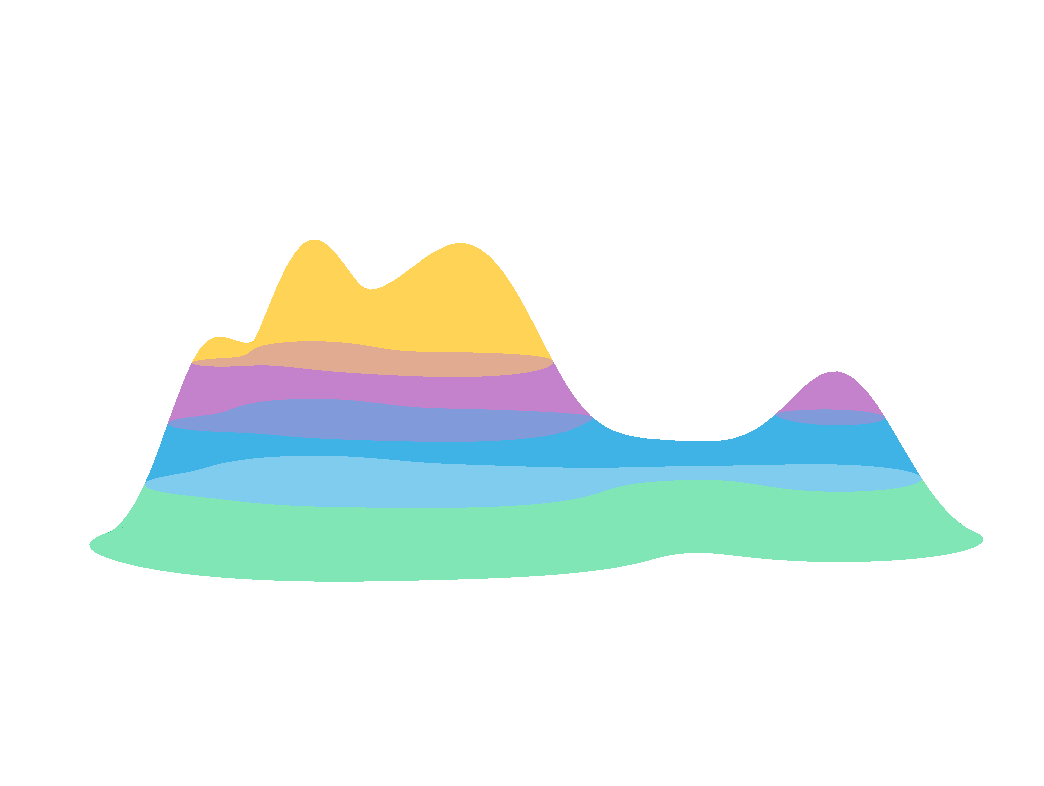
\includegraphics[trim=50 190 0 200, clip, scale=0.2]{scripts/figures/scalar.png}
  % 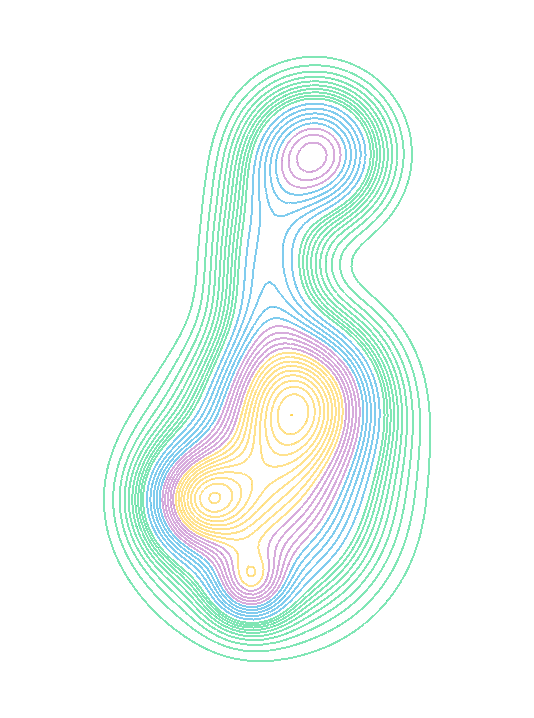
\includegraphics[trim=100 25 75 0, clip, angle=280, scale=0.25]{scripts/figures/scalar_contour.png}
  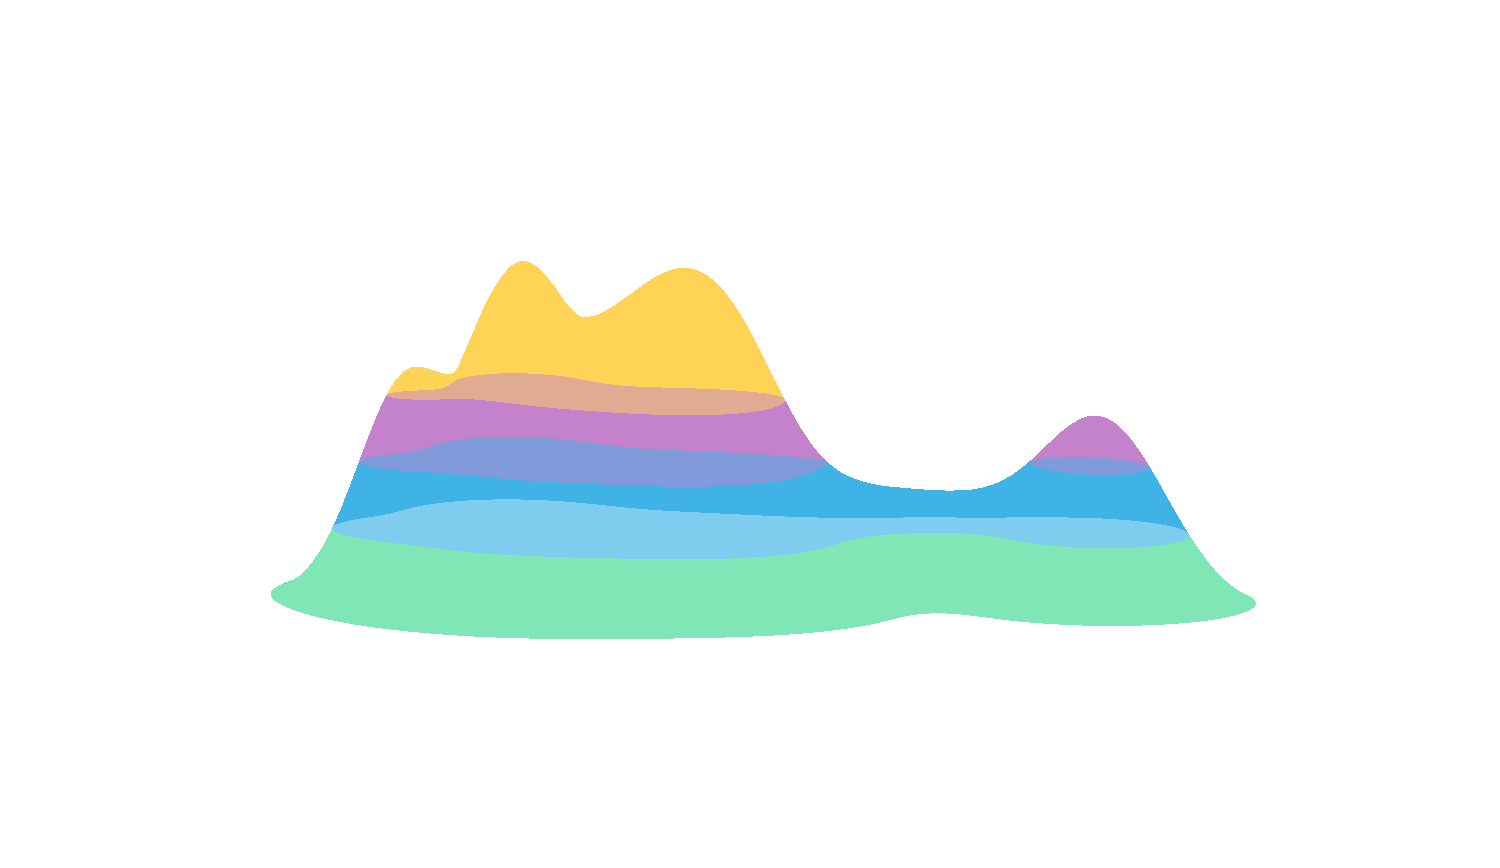
\includegraphics[trim=200 200 200 200, clip, width=0.5\textwidth]{scripts/figures/surf/side.png}
  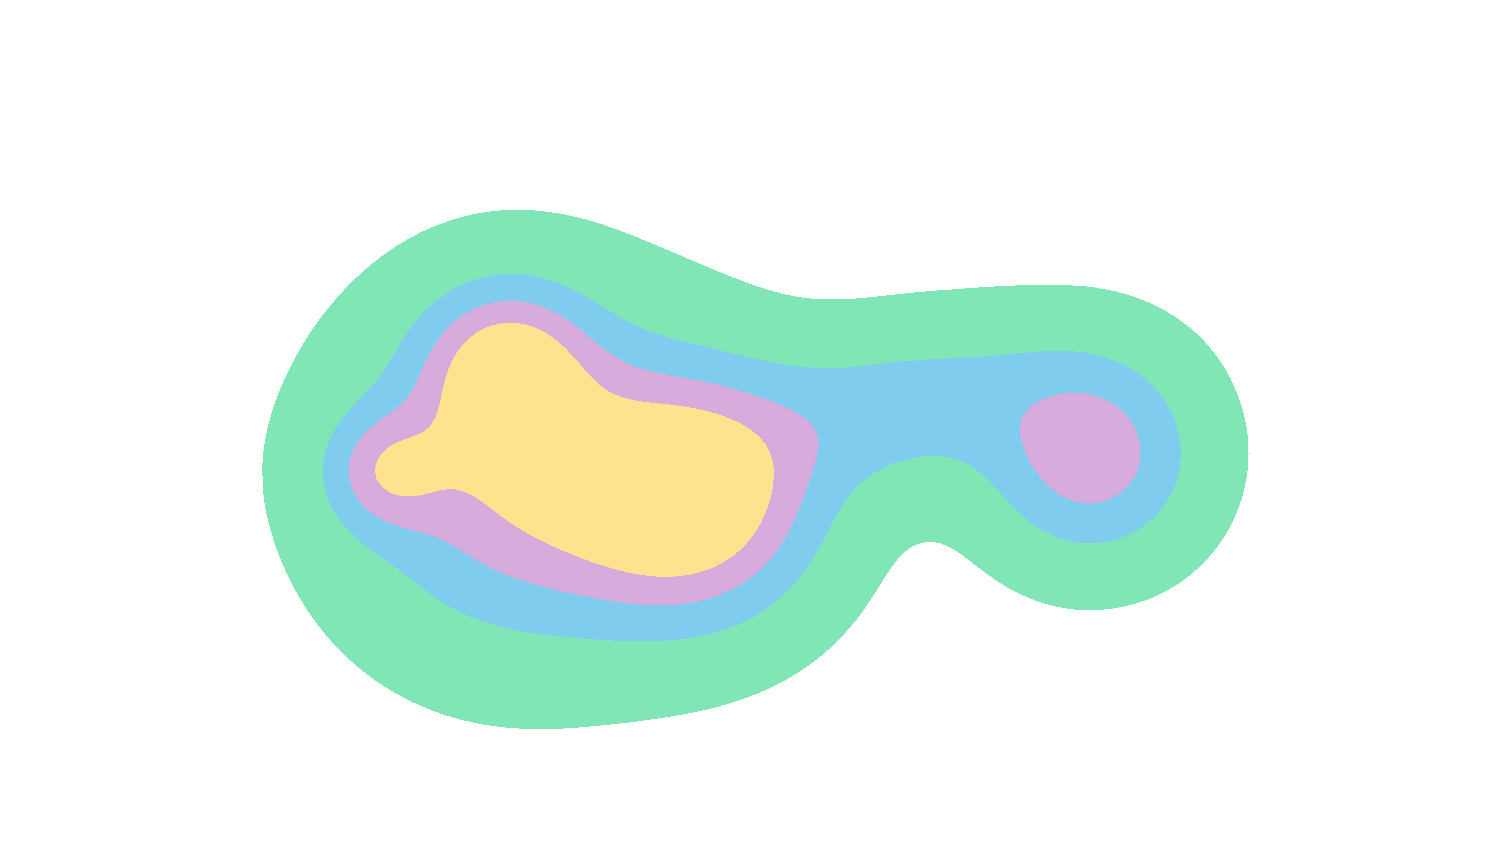
\includegraphics[trim=200 0 200 200, clip, width=0.3\textwidth]{scripts/figures/surf/top.png}
  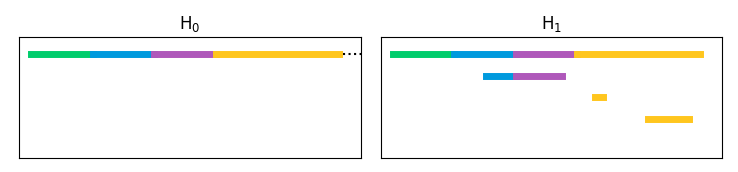
\includegraphics[scale=0.75]{scripts/figures/scalar_barcode_true.png}
  % \includegraphics[trim=0 310 270 0, clip, scale=0.8]{scripts/figures/scalar_restricted.png}
  % \includegraphics[scale=0.55]{scripts/figures/scalar_barcode_super_0.png}
  % \includegraphics[scale=0.55]{scripts/figures/scalar_barcode_sub_1.png}
\end{figure}

% \begin{figure}\label{fig:restricted}
%   \centering
%   \includegraphics[scale=0.6]{scripts/figures/scalar_restricted.png}
%   \caption{Persistence barcodes in dimension 0, 1, and 2 (horizonal axis) of the function depicted in Figure~\ref{fig:scalar} (top row) as well as the function \emph{restricted} to the region above the green, blue, and purple sub-levelsets (rows 2-4 respectively).}
% \end{figure}
% \begin{figure}\label{fig:truncated}
%   \centering
%   \includegraphics[trim=0 0 0 125, clip, scale=0.6]{scripts/figures/scalar_truncated.png}
%     \caption{The persistent homology taken relative to the green, blue, and purple sub-levelsets, respectively.}
% \end{figure}
